\documentclass[12pt,a4paper]{article}

% ── Packages ──────────────────────────────────────────────────────────────────
\usepackage[T1]{fontenc}
\usepackage[utf8]{inputenc}
\usepackage[english]{babel}
\usepackage{geometry}
\usepackage{setspace}
\usepackage{microtype}
\usepackage{parskip}
\usepackage{graphicx}
\usepackage{xcolor}
\usepackage{booktabs}
\usepackage{longtable}
\usepackage{tabularx}
\usepackage{array}
\usepackage{float}
\usepackage{caption}
\usepackage{subcaption}
\usepackage{fancyhdr}
\usepackage{titlesec}
\usepackage{enumitem}
\usepackage{tcolorbox}
\usepackage{tikz}
\usepackage{multirow}
\usepackage{hyperref}

% ── Geometry ──────────────────────────────────────────────────────────────────
\geometry{a4paper, top=2cm, bottom=2cm, left=2cm, right=2cm, headheight=15pt}

% ── Color Palette ─────────────────────────────────────────────────────────────
\definecolor{helixpurple}{HTML}{3C3489}
\definecolor{helixpurplelight}{HTML}{EEEDFE}
\definecolor{helixpurplemid}{HTML}{5A50B0}
\definecolor{helixteal}{HTML}{0F6E56}
\definecolor{helixteallight}{HTML}{E1F5EE}
\definecolor{helixamber}{HTML}{7A4A00}
\definecolor{helixamberlight}{HTML}{FDF3DC}
\definecolor{helixgray}{HTML}{3A3A38}
\definecolor{helixgraylight}{HTML}{F4F3EF}
\definecolor{helixborder}{HTML}{CCCAC0}
\definecolor{textprimary}{HTML}{1E1E1C}
\definecolor{textsecondary}{HTML}{5A5958}

% ── tcolorbox Styles ──────────────────────────────────────────────────────────
\tcbuselibrary{skins,breakable}

\newtcolorbox{infobox}[1][]{
	enhanced, breakable,
	colback=helixpurplelight, colframe=helixpurple,
	fonttitle=\bfseries\small\color{helixpurple},
	left=10pt, right=10pt, top=7pt, bottom=7pt,
	arc=5pt, boxrule=0.6pt, #1
}

\newtcolorbox{successbox}[1][]{
	enhanced, breakable,
	colback=helixteallight, colframe=helixteal,
	fonttitle=\bfseries\small\color{helixteal},
	left=10pt, right=10pt, top=7pt, bottom=7pt,
	arc=5pt, boxrule=0.6pt, #1
}

\newtcolorbox{warningbox}[1][]{
	enhanced, breakable,
	colback=helixamberlight, colframe=helixamber,
	fonttitle=\bfseries\small\color{helixamber},
	left=10pt, right=10pt, top=7pt, bottom=7pt,
	arc=5pt, boxrule=0.6pt, #1
}

\newtcolorbox{sectionbox}[1][]{
	enhanced, breakable,
	colback=helixgraylight, colframe=helixborder,
	left=10pt, right=10pt, top=7pt, bottom=7pt,
	arc=5pt, boxrule=0.5pt, #1
}

% ── Hyperref ──────────────────────────────────────────────────────────────────
\hypersetup{
	colorlinks=true,
	linkcolor=helixpurple,
	urlcolor=helixteal,
	citecolor=helixgray,
	pdftitle={HELIX PoC -- Software Design Document},
	pdfauthor={Yasseene -- Tek-Up University},
	pdfsubject={PoC Cybersecurity Platform SDD}
}

% ── Section Styling ───────────────────────────────────────────────────────────
\titleformat{\section}[block]
{\normalfont\LARGE\bfseries\color{helixpurple}}
{\thesection.}{12pt}{}
[\vspace{3pt}\color{helixborder}\rule{\linewidth}{0.6pt}\vspace{6pt}]

\titleformat{\subsection}
{\normalfont\large\bfseries\color{helixgray}}
{\thesubsection}{10pt}{}

\titleformat{\subsubsection}
{\normalfont\normalsize\bfseries\color{textsecondary}}
{\thesubsubsection}{8pt}{}

\titlespacing*{\section}{0pt}{10pt}{22pt}
\titlespacing*{\subsection}{0pt}{18pt}{8pt}
\titlespacing*{\subsubsection}{0pt}{12pt}{5pt}

% ── Header / Footer ───────────────────────────────────────────────────────────
\pagestyle{fancy}
\fancyhf{}
\renewcommand{\headrulewidth}{0.4pt}
\renewcommand{\footrulewidth}{0.4pt}
\fancyhead[L]{\small\color{textsecondary}\scshape{HELIX Platform}}
\fancyhead[R]{\small\color{textsecondary}Software Design Document}
\fancyfoot[C]{\small\color{textsecondary}\thepage}
\fancyfoot[R]{\small\color{textsecondary}2025--2026}

% ── Diagram insertion helpers ─────────────────────────────────────────────────
\newcommand{\diagramfigure}[3]{%
  \begin{figure}[H]
    \centering
    \includegraphics[width=0.98\linewidth,height=0.88\textheight,keepaspectratio]{#1}
    \caption{#2}
    \label{#3}
  \end{figure}%
}

\newcommand{\rotatedportraitdiagram}[3]{%
  \clearpage
  \begin{figure}[p]
    \centering
    \includegraphics[angle=90,width=0.92\textheight,height=0.84\textwidth,keepaspectratio]{#1}
    \caption{#2}
    \label{#3}
  \end{figure}%
  \clearpage
}

\newcommand{\fullportraitdiagram}[3]{%
  \clearpage
  \begin{figure}[p]
    \centering
    \includegraphics[width=0.96\linewidth,height=0.90\textheight,keepaspectratio]{#1}
    \caption{#2}
    \label{#3}
  \end{figure}%
  \clearpage
}

% ── Table Column Types ────────────────────────────────────────────────────────
\newcolumntype{L}[1]{>{\raggedright\arraybackslash}p{#1}}
\newcolumntype{C}[1]{>{\centering\arraybackslash}p{#1}}

\setlist[itemize]{leftmargin=1.5em, itemsep=4pt, topsep=5pt}
\setlist[enumerate]{leftmargin=1.7em, itemsep=4pt, topsep=5pt}

% ══════════════════════════════════════════════════════════════════════════════
\begin{document}
	\setstretch{1.25}

% ── Title page ────────────────────────────────────────────────────────────────
\pagenumbering{gobble}
\begin{titlepage}
	\thispagestyle{empty}
	\noindent\colorbox{helixpurple}{%
		\parbox{\dimexpr\textwidth+2\fboxsep\relax}{%
			\vspace{10pt}
			\hspace{8pt}\textcolor{white}{\small\scshape{Software Design Document --- PoC Version}}%
			\vspace{10pt}
		}%
	}
	\vspace{2cm}
	\begin{center}
		{\fontsize{52}{60}\selectfont\bfseries\color{helixpurple} HELIX}\\[10pt]
		{\Large\color{textsecondary}Cybersecurity Operations Platform --- Proof of Concept}\\[8pt]
		{\normalsize\color{helixpurplemid}\textit{Architecture $\cdot$ Design $\cdot$ UML Documentation}}\\[20pt]
		\color{helixborder}\rule{0.65\textwidth}{0.5pt}\\[25pt]
		{\fontsize{22}{28}\selectfont\bfseries\color{helixpurple} Software Design Document}\\[4pt]
		{\large\color{helixpurplemid}Cahier des Charges Technique}
	\end{center}
	\vspace{1.5cm}
	\begin{center}
		\begin{tabular}{L{5.2cm} L{7.5cm}}
			\toprule
			\textbf{Author}         & Yasseene \\
			\midrule
			\textbf{Institution}    & Tek-Up University, Ariana, Tunisia \\
			\midrule
			\textbf{Academic Year}  & 2025 -- 2026 \\
			\midrule
			\textbf{Version}        & 1.0 -- Proof of Concept \\
			\midrule
			\textbf{Classification} & Academic --- Confidential \\
			\midrule
			\textbf{Repository}     & \texttt{github.com/mUchiha26/HELIX-PoC} \\
			\midrule
			\textbf{Date}           & June 2026 \\
			\bottomrule
		\end{tabular}
	\end{center}
	\vfill
	\begin{center}
		{\small Submitted in partial fulfilment of the requirements for the degree of\\
		Bachelor of Engineering in Computer Science (Cybersecurity Track)}
	\end{center}
	\vfill
	\noindent\colorbox{helixgraylight}{%
		\parbox{\dimexpr\textwidth+2\fboxsep\relax}{%
			\vspace{8pt}
			\hspace{8pt}\small\color{textsecondary}%
			Tek-Up University \hfill Ariana, Tunisia \hfill Academic Year 2025--2026
			\vspace{8pt}
		}%
	}
\end{titlepage}
\clearpage
\pagenumbering{arabic}

% ── TOC ───────────────────────────────────────────────────────────────────────
\tableofcontents
\newpage

% ══════════════════════════════════════════════════════════════════════════════
\section{Introduction}

\subsection{Project Overview}
HELIX is a modular cybersecurity operations platform that unifies four operational
domains within a single authenticated environment: Blue Team defensive monitoring,
Red Team offensive testing, AI-assisted threat analysis, and machine-learning anomaly
detection. This Software Design Document (SDD) defines the architectural and design
specifications for the Proof of Concept (PoC) phase, covering static structure,
dynamic behaviour, deployment topology, and all major UML artefacts.

\subsection{Context and Problem Statement}
Global cybercrime costs continue to rise whilst security education environments
remain fragmented across disjoint tools --- separate SIEMs, scanners, AI assistants,
and training platforms each requiring distinct credentials, data models, and skill sets.
Students and early-career professionals consequently lack holistic, realistic environments
for developing combined defensive and offensive competencies.

\textit{How to design and implement a unified, accessible cybersecurity platform that
combines threat monitoring, AI-assisted analysis, and ML anomaly detection for academic
and training purposes, while maintaining a modular architecture for future enterprise
evolution?}

\subsection{Objectives}
\begin{itemize}[leftmargin=*,itemsep=2pt]
  \item \textbf{General:} Deliver a functional PoC demonstrating end-to-end platform
    viability within a unified web interface deployable on a standard XAMPP stack.
  \item \textbf{Functional:} Implement RBAC authentication, centralised dashboards,
    log ingestion, alert visualisation, ML anomaly scoring (Isolation Forest), AI-powered
    alert explanation (OpenAI API), and a Red Team network port scanner.
  \item \textbf{Academic:} Demonstrate the full software engineering lifecycle,
    multi-language integration (PHP, Python, Java, JavaScript), and produce a
    comprehensive UML documentation suite.
\end{itemize}

\subsection{Scope}
The PoC covers seven core modules: Authentication \& RBAC, Security Dashboard,
Log Ingestion, Alert Visualisation, ML Anomaly Detection, AI Assistant, and the
Red Team Port Scanner. Advanced exploitation frameworks, microservice orchestration,
real-time streaming, and multi-tenancy are deferred to the MVP and production phases.

% ══════════════════════════════════════════════════════════════════════════════
\section{Technology Stack}

The stack was selected to maximise accessibility and academic reproducibility whilst
supporting all required capabilities.

\begin{table}[H]
  \centering
  \renewcommand{\arraystretch}{1.3}
  \begin{tabular}{@{}L{2.8cm} L{3.4cm} p{7.5cm}@{}}
    \toprule
    \textbf{Layer} & \textbf{Technology} & \textbf{Role and Justification} \\
    \midrule
    Frontend
      & HTML5, CSS3, JavaScript
      & Role-appropriate dashboards, data charts, and alert views.
        No framework required; served directly by Apache. \\
    Backend / API
      & PHP 8.x + Composer
      & RESTful API, session management, RBAC enforcement,
        and orchestration of ML / AI sub-services. \\
    Database
      & MySQL 8.x (XAMPP)
      & Relational persistence for users, logs, alerts,
        anomaly scores, chat history, and scan results. \\
    ML Service
      & Python 3.x, scikit-learn
      & Isolation Forest unsupervised anomaly detection;
        invoked by PHP via \texttt{shell\_exec()}. \\
    Java Module
      & Java JDK
      & Hash scanning and log-parsing utilities;
        invoked by PHP \texttt{JavaBridge} service. \\
    AI Integration
      & OpenAI API
      & Natural-language alert explanation and
        remediation guidance over HTTPS. \\
    Server / Env.
      & Apache 2.x (XAMPP)
      & Local development and PoC deployment environment. \\
    \bottomrule
  \end{tabular}
  \caption{HELIX PoC Technology Stack}
\end{table}

The PHP backend follows a strict layered architecture: Front Controller $\to$
Middleware (\texttt{AuthMiddleware}, \texttt{RoleMiddleware}) $\to$ Controllers
$\to$ Services $\to$ Models $\to$ PDO/MySQL. Composer provides PSR-4 autoloading.
No layer may be skipped; controllers never access the database directly.

% ══════════════════════════════════════════════════════════════════════════════
\section{Requirements Analysis}

\subsection{Functional Requirements Summary}
\begin{table}[H]
  \centering
  \renewcommand{\arraystretch}{1.25}
  \begin{tabular}{@{}L{1.4cm} L{3.6cm} p{8.6cm}@{}}
    \toprule
    \textbf{IDs} & \textbf{Module} & \textbf{Key Requirements} \\
    \midrule
    FR-001--007
      & Authentication \& RBAC
      & Registration, bcrypt login ($\geq$cost 10), session management,
        role assignment, account enable/disable, admin user management. \\
    FR-010--014
      & Dashboard
      & Aggregated statistics, severity charts, time-series views,
        role-filtered metrics. \\
    FR-020--024
      & Log Ingestion
      & CSV/TXT upload, field parsing, bulk DB insertion,
        duplicate detection, ingestion summary. \\
    FR-030--034
      & Alert Visualisation
      & Severity-coded listing (Critical/High/Medium/Low),
        filter by source/time, acknowledgement workflow. \\
    FR-040--044
      & ML Anomaly Detection
      & Isolation Forest scoring on event frequency, error rate,
        IP diversity; threshold-based alert generation; score history. \\
    FR-050--054
      & AI Assistant
      & Multi-turn conversational analysis, alert context attachment,
        remediation suggestions, session persistence. \\
    FR-060--063
      & Red Team Tools
      & Port scan with target/range specification, result persistence,
        scan history; restricted to Red/Purple Team roles. \\
    \bottomrule
  \end{tabular}
  \caption{Functional Requirements by Module}
\end{table}

\subsection{Non-Functional Requirements Summary}
\begin{table}[H]
  \centering
  \renewcommand{\arraystretch}{1.25}
  \begin{tabular}{@{}L{3cm} p{11.2cm}@{}}
    \toprule
    \textbf{Category} & \textbf{Specification} \\
    \midrule
    Performance
      & Dashboard loads $<2$s (1,000 entries); ML scoring $<5$s (500 entries);
        AI response $<8$s. API endpoints $<2$s under normal PoC load. \\
    Security
      & bcrypt hashing (cost $\geq 10$); PDO parameterised queries (SQL injection
        prevention); server-side PHP sessions; no sensitive data in client storage. \\
    Maintainability
      & Strict Controller $\to$ Service $\to$ Model hierarchy; PSR-4 namespacing;
        documented API endpoints; no layer skipping. \\
    Deployability
      & Single XAMPP installation; no containerisation required for PoC phase;
        Python and Java JDK as explicit prerequisites. \\
    \bottomrule
  \end{tabular}
  \caption{Non-Functional Requirements Summary}
\end{table}

\subsection{User Roles and Permissions}
\begin{table}[H]
  \centering
  \renewcommand{\arraystretch}{1.25}
  \begin{tabular}{@{}L{3.4cm} L{2.8cm} p{8cm}@{}}
    \toprule
    \textbf{Actor} & \textbf{Type} & \textbf{Core Permissions} \\
    \midrule
    Visitor                & Unauthenticated  & Browse public content, register, log in. \\
    Learner                & Human            & Study materials, personal notes, read-only alerts, AI assistant. \\
    Blue Team Operator     & Human            & Dashboard, log ingestion, alert management, ML scores, AI assistant. \\
    Red Team Operator      & Human            & Port scanner, scan results, writeup publishing. \\
    Purple Team Operator   & Human (hybrid)   & Combined Blue + Red capabilities, cross-correlation. \\
    Administrator          & Human            & Full access: user management, system configuration, all modules. \\
    Detection Engine       & System actor     & Autonomous ML scoring and alert generation (no user interaction). \\
    \bottomrule
  \end{tabular}
  \caption{User Roles and System Actors}
\end{table}

% ══════════════════════════════════════════════════════════════════════════════
\section{Use Case Modelling}

\subsection{Global Use Case Diagram}

The following diagram captures all 33 use cases across seven functional packages,
all eight actors, and the complete set of \texttt{<<include>>} and \texttt{<<extend>>}
relationships. It is rendered on a dedicated portrait page to preserve readability
(see Figure~\ref{fig:usecase_detailed}).

\fullportraitdiagram%
  {UML/use_case/usecase.png}%
  {HELIX PoC --- Global Use Case Diagram (all actors, all 33 UCs, all relationships)}%
  {fig:usecase_detailed}

\subsection{Major Use Case Descriptions}

\textbf{UC-02: Log In}
\begin{infobox}
\textbf{Actors:} Visitor (initiates); Authenticated User (post-condition).
\quad\textbf{Preconditions:} Active account exists.\\
\textbf{Main Flow:} Submit credentials $\to$ Validate bcrypt hash $\to$ Create PHP
session with role $\to$ Redirect to role-appropriate dashboard.\\
\textbf{Alt Flow:} Invalid credentials return HTTP 401 (no field disambiguation).
\quad\textbf{Postconditions:} Authenticated session established.
\end{infobox}

\textbf{UC-11: Automated Detection}
\begin{infobox}
\textbf{Actors:} Detection Engine (system actor).
\quad\textbf{Preconditions:} Log entries have been ingested.\\
\textbf{Main Flow:} Trigger $\to$ \textit{Ingest Logs} (UC-12) $\to$
\textit{Pre-filter Noise} (UC-13) $\to$ \textit{Score via ML} (UC-14/16) $\to$
\textit{Generate Alerts} (UC-15) for HIGH/CRITICAL scores.\\
\textbf{Alt Flow:} ML service unavailable --- entries queued for deferred scoring.
\quad\textbf{Postconditions:} Alerts generated and persisted.
\end{infobox}

\textbf{UC-17: Run Reconnaissance}
\begin{infobox}
\textbf{Actors:} Red Team Operator, Purple Team Operator.
\quad\textbf{Preconditions:} Authenticated; target and port range specified.\\
\textbf{Main Flow:} Submit parameters $\to$ \texttt{JavaBridge} invokes Java scanner
via \texttt{shell\_exec()} $\to$ Parse output $\to$ Persist in \texttt{scan\_results}.\\
\textbf{Alt Flow:} Unreachable target returns error; nothing persisted.
\quad\textbf{Postconditions:} Scan results stored and visible in history.
\end{infobox}

\textbf{UC-31: Use AI Assistant}
\begin{infobox}
\textbf{Actors:} All authenticated roles.
\quad\textbf{Preconditions:} Authenticated; OpenAI API key configured.\\
\textbf{Main Flow:} Submit message (optionally with alert context) $\to$
Retrieve conversation history $\to$ Build prompt $\to$ Call OpenAI API $\to$
Persist and return response (\textit{includes} UC-32: Reliable Fixes,
UC-33: Suggest Attack Methods).\\
\textbf{Alt Flow:} API unavailable --- degraded-mode message; session preserved.
\quad\textbf{Postconditions:} Guidance persisted; multi-turn conversation maintained.
\end{infobox}

% ══════════════════════════════════════════════════════════════════════════════
\section{Static Design}

\subsection{Class Diagram}

The class diagram (Figure~\ref{fig:class_diagram}) covers all major architectural
layers: Config, Middleware, Controllers, Services, Models, and Helpers. The strict
dependency direction (Controller $\to$ Service $\to$ Model $\to$ Database) is
enforced throughout.

\fullportraitdiagram%
  {UML/class/class.png}%
  {HELIX PoC --- Class Diagram }%
  {fig:class_diagram}

\subsection{Main Classes and Responsibilities}

\begin{itemize}[leftmargin=*,itemsep=3pt]
  \item \textbf{User} --- Central entity. Attributes: \texttt{id, username, email,
    password\_hash, role, status}. Operations: \texttt{findByUsername()},
    \texttt{create()}, \texttt{updateRole()}, \texttt{toggleStatus()}.
    Extended by role-specific sub-entities.

  \item \textbf{LogEntry} --- Parsed log record. Attributes: \texttt{id, timestamp,
    source\_ip, severity, raw\_message, parsed\_fields}. Supports
    \texttt{bulkInsert()} for CSV batch ingestion.

  \item \textbf{Alert} --- Generated from anomalous LogEntries. Attributes:
    \texttt{id, log\_entry\_id, severity\_score, status}
    (Open / Investigating / Resolved), \texttt{created\_at}.

  \item \textbf{AnomalyScore} --- Persists ML detection results. Attributes:
    \texttt{id, log\_entry\_id, score, model\_version}. Links to \texttt{LogEntry}
    by foreign key.

  \item \textbf{AIService} --- Constructs multi-turn OpenAI prompts from
    \texttt{ChatSession} history, calls the external API, and persists responses
    in \texttt{ChatMessage}.

  \item \textbf{JavaBridge} --- PHP-to-Java interoperability layer. Constructs
    \texttt{shell\_exec()} commands for the compiled Java module and parses stdout.

  \item \textbf{ScanResult} --- Stores port scanner output. Attributes:
    \texttt{id, target\_ip, port, protocol, status, scan\_date, operator\_id}.
\end{itemize}

\textbf{Key relationships:}
\textbf{User} $1 \to *$ \textbf{Alert} (operator manages alerts);
\textbf{LogEntry} $1 \to 0..1$ \textbf{AnomalyScore};
\textbf{AnomalyScore} $1 \to 0..1$ \textbf{Alert};
\textbf{User} $1 \to *$ \textbf{ScanResult};
\textbf{ChatSession} $1 \to *$ \textbf{ChatMessage}.

% ══════════════════════════════════════════════════════════════════════════════
\section{Dynamic Design}

All five sequence diagrams share a common structure: Browser $\to$ \texttt{index.php}
(front controller) $\to$ Middleware $\to$ Controller $\to$ Service $\to$ Model $\to$
MySQL, with external calls to Python, Java, or the OpenAI API where applicable.

\subsection{Authentication Workflow}

\diagramfigure%
  {UML/sequence/sequence_auth.png}%
  {Sequence Diagram: Authentication and Role-Based Session Establishment}%
  {fig:seq_auth}

The user submits credentials to \texttt{POST /auth/login}. \texttt{AuthService}
queries \texttt{User::findByUsername()} via PDO, verifies the bcrypt hash with
\texttt{password\_verify()}, and populates the PHP session with the user ID and role.
On failure, HTTP 401 is returned with no field-specific information.

\subsection{Security Dashboard and Event Monitoring}

\diagramfigure%
  {UML/sequence/sequence_dashboard.png}%
  {Sequence Diagram: Security Dashboard and Event Monitoring}%
  {fig:seq_dashboard}

The dashboard sequence captures role-aware metrics aggregation, alert summaries,
and filtered event queries. It is kept on a portrait page because the rendered asset
is tall rather than wide.

\subsection{Log Ingestion and ML Detection Pipeline}

\diagramfigure%
  {UML/sequence/sequence_detection_pipeline.png}%
  {Sequence Diagram: Log Ingestion and Automated Detection Pipeline}%
  {fig:seq_ml}

The operator uploads a CSV/TXT file. After role validation, the ingestion service
parses rows, stores them, and runs the detection cycle. The backend then invokes
the Python detection script via \texttt{shell\_exec()}, passing feature vectors
as JSON. Python applies Isolation Forest, returns scores to stdout, and the PHP
layer persists them via \texttt{AnomalyScore::insertBatch()}. Entries exceeding the
HIGH/CRITICAL threshold trigger \texttt{Alert::create()}.

\subsection{AI Assistant Workflow}

\diagramfigure%
  {UML/sequence/sequence_ai_assistant.png}%
  {Sequence Diagram: AI Assistant --- OpenAI API Multi-Turn Interaction}%
  {fig:seq_ai}

The user sends a message with optional alert context. \texttt{AIService} retrieves
conversation history from \texttt{ChatMessage}, constructs a multi-turn prompt with
a cybersecurity-specialist system role, and dispatches an HTTPS call to the
OpenAI API. The response is simultaneously returned to the frontend and persisted.

\subsection{Red Team Reconnaissance Workflow}

\diagramfigure%
  {UML/sequence/sequence_red_team_recon.png}%
  {Sequence Diagram: Red Team Port Scanner --- Java Module Execution}%
  {fig:seq_redteam}

An authorised Red or Purple Team operator submits a target IP and port range.
\texttt{JavaBridge::execute()} constructs a \texttt{java -cp \ldots{} PortScanner}
command via \texttt{shell\_exec()}. The Java module scans and writes structured
results to stdout; the bridge persists them in \texttt{ScanResult}.

% ══════════════════════════════════════════════════════════════════════════════
\section{Business Process Modelling}

The three activity diagrams below model the principal operational workflows.
Each rendered PNG is placed on its own page because the generated diagrams are
already optimized for readability rather than compactness.

\diagramfigure%
  {UML/activity/activity_auth.png}%
  {Activity: Authentication Process}%
  {fig:act_auth}

\textbf{Authentication (Figure~\ref{fig:act_auth}):} Three sequential guard conditions
--- input validation, user lookup, bcrypt verification. Any failure produces a generic
error (no field disambiguation). Success initialises the PHP session.

\diagramfigure%
  {UML/activity/activity_alert_lifecycle.png}%
  {Activity: Alert Lifecycle and Triage Process}%
  {fig:act_alert}

\textbf{Alert Lifecycle (Figure~\ref{fig:act_alert}):} This workflow covers
acknowledgement, investigation, escalation, and resolution. It complements the
detection pipeline by showing how generated alerts move through analyst review.

\diagramfigure%
  {UML/activity/activity_detection_pipeline.png}%
  {Activity Diagram: Log Ingestion and Automated Detection Pipeline}%
  {fig:act_logdetect}

\textbf{Detection Pipeline (Figure~\ref{fig:act_logdetect}):} After ingestion, the
flow forks --- database persistence and ML scoring proceed concurrently. Entries
exceeding the anomaly threshold follow the alert generation branch; compliant entries
are marked scored. A deferred-scoring path handles ML service unavailability.

% ══════════════════════════════════════════════════════════════════════════════
\section{Software Architecture}

\subsection{Architectural Overview}
The HELIX PoC follows a \textbf{Modular Monolith} architecture with clear service
boundaries, designed for simplicity in the PoC phase whilst enabling seamless extraction
of the ML, AI, and Java services into independent microservices for the MVP phase.

\begin{figure}[H]
\centering
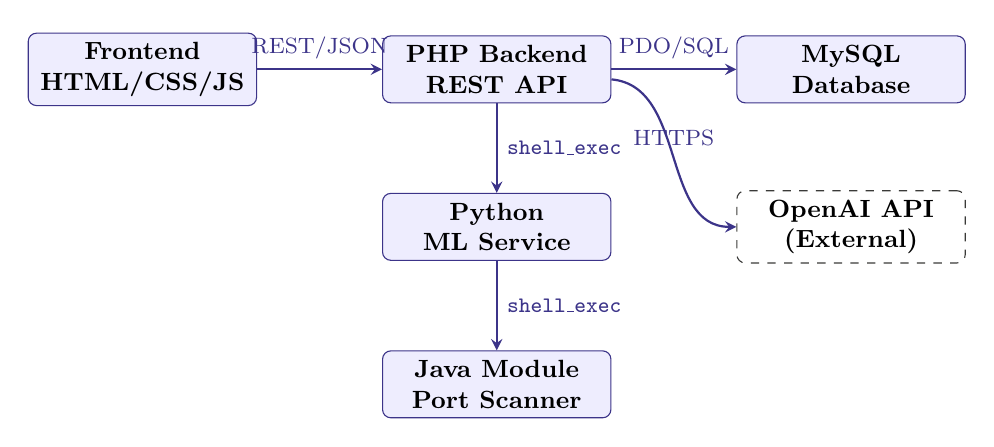
\begin{tikzpicture}[
  box/.style={rectangle,draw=helixpurple,rounded corners=3pt,
    fill=helixpurplelight,minimum width=2.9cm,minimum height=0.85cm,
    align=center,font=\small\bfseries},
  ext/.style={rectangle,draw=helixgray,rounded corners=3pt,
    fill=white,minimum width=2.9cm,minimum height=0.85cm,
    align=center,font=\small\bfseries,dashed},
  arr/.style={->,>=stealth,thick,color=helixpurple}
]
  \node[box] (fe)   at (0,0)    {Frontend\\HTML/CSS/JS};
  \node[box] (be)   at (4.5,0)  {PHP Backend\\REST API};
  \node[box] (db)   at (9,0)    {MySQL\\Database};
  \node[box] (py)   at (4.5,-2) {Python\\ML Service};
  \node[box] (java) at (4.5,-4) {Java Module\\Port Scanner};
  \node[ext] (oai)  at (9,-2)   {OpenAI API\\(External)};

  \draw[arr] (fe)   -- node[above,font=\footnotesize]{REST/JSON}   (be);
  \draw[arr] (be)   -- node[above,font=\footnotesize]{PDO/SQL}     (db);
  \draw[arr] (be)   -- node[right,font=\footnotesize]{\texttt{shell\_exec}} (py);
  \draw[arr] (py)   -- node[right,font=\footnotesize]{\texttt{shell\_exec}} (java);
  \draw[arr] (be) to[out=-5,in=180] node[above,font=\footnotesize]{HTTPS} (oai);
\end{tikzpicture}
\caption{Component Interaction Overview --- HELIX PoC}
\label{fig:components}
\end{figure}

\subsection{Major Components}

\begin{enumerate}[leftmargin=*,itemsep=3pt]
  \item \textbf{Presentation Layer:} HTML/CSS/JS frontend providing role-based
    dashboards, alert views, log upload forms, and AI chat interface. Communicates
    exclusively with the PHP backend via the JSON REST API.

  \item \textbf{Application Layer (PHP):} Layered REST API. Handles HTTP requests,
    session management, RBAC enforcement via middleware, and orchestration of
    calls to external services. Provides the \texttt{JavaBridge} abstraction for
    subprocess-based integrations.

  \item \textbf{Data Layer (MySQL):} Seven relational tables:
    \texttt{users}, \texttt{log\_entries}, \texttt{alerts},
    \texttt{anomaly\_scores}, \texttt{chat\_sessions}, \texttt{chat\_messages},
    \texttt{scan\_results}. All queries use PDO parameterised statements.

  \item \textbf{ML Service (Python):} Standalone script (\texttt{ml\_service/detect.py})
    invoked synchronously via \texttt{shell\_exec()}. Applies the Isolation Forest
    model to log feature vectors and returns anomaly scores as JSON to stdout.

  \item \textbf{AI Service (External):} OpenAI Chat Completions API. Called from
    \texttt{AIService} with a system prompt, conversation history, and user message.
    Responses are persisted in \texttt{chat\_messages} for multi-turn continuity.

  \item \textbf{Red Team Module (Java):} Compiled Java class files invoked through
    \texttt{JavaBridge}. Performs port scanning and hash analysis with structured
    stdout output captured and persisted by the PHP layer.
\end{enumerate}

\textbf{Interaction principle:} The PHP backend is the sole orchestrator. Neither the
frontend nor subprocess modules access MySQL directly. All inter-service communication
is mediated by the service layer, ensuring consistent audit logging, input validation,
and data formatting before persistence.

% ══════════════════════════════════════════════════════════════════════════════
\section{Deployment Architecture}

\diagramfigure%
  {UML/deployment/deployment.png}%
  {Deployment Diagram: PoC Execution Environment and Node Topology}%
  {fig:deployment}

\subsection{Execution Environment and Node Responsibilities}
\begin{itemize}[leftmargin=*,itemsep=3pt]
  \item \textbf{Client Node:} Any modern web browser (Chrome, Firefox, Edge)
    accessing \texttt{http://helix.local} or \texttt{http://localhost/HELIX}.
    Renders the frontend interface and sends HTTP/JSON requests to the backend.

  \item \textbf{Application Server (XAMPP / localhost):} Hosts Apache 2.x, PHP 8.x,
    the HELIX application code, the Python runtime, and the Java JDK. Manages
    all user sessions, API routing, and subprocess invocations. MySQL 8.x
    co-located on the same node in the PoC configuration.

  \item \textbf{Database Server (MySQL):} Co-located with the application server.
    Stores all persistent data; accessible only from \texttt{localhost} (no external
    network exposure).

  \item \textbf{ML Execution Environment:} Python 3.x with scikit-learn and pandas,
    installed on the same server node. Invoked synchronously on demand --- no
    persistent process or queue required.

  \item \textbf{External Cloud Services:} OpenAI API (\texttt{api.openai.com})
    accessed via HTTPS from the PHP backend. The only external runtime dependency;
    requires an active internet connection and a valid API key stored in
    \texttt{.env}.
\end{itemize}

\begin{table}[H]
  \centering
  \renewcommand{\arraystretch}{1.25}
  \begin{tabular}{@{}L{3cm} L{3cm} L{2.8cm} p{4.8cm}@{}}
    \toprule
    \textbf{Source} & \textbf{Target} & \textbf{Protocol} & \textbf{Notes} \\
    \midrule
    Browser            & Apache/PHP       & HTTP/1.1               & REST JSON; session via cookie \\
    PHP                & MySQL            & TCP/3306 (PDO)         & Parameterised queries; localhost only \\
    PHP                & Python ML        & \texttt{shell\_exec}   & JSON via stdin/stdout; synchronous \\
    PHP                & Java Module      & \texttt{shell\_exec}   & Args + stdout; synchronous \\
    PHP                & OpenAI API       & HTTPS/443              & API key in Authorization header \\
    \bottomrule
  \end{tabular}
  \caption{Inter-Node Communication Protocols}
\end{table}

% ══════════════════════════════════════════════════════════════════════════════
\section{Conclusion}

\subsection{Summary of the PoC}
The HELIX Proof of Concept delivers a fully functional, multi-module cybersecurity
operations platform across seven integrated capabilities --- authentication and RBAC,
security dashboard, log ingestion, alert visualisation, ML anomaly detection,
AI-assisted analysis, and Red Team orchestration. The platform is implemented on a
deliberately accessible stack (PHP, MySQL, Python, Java) deployable on a single XAMPP
server, demonstrating that architectural coherence and academic rigour need not depend
on complex infrastructure.

\subsection{Achieved Objectives}
\begin{itemize}[leftmargin=*,itemsep=2pt]
  \item Implemented robust RBAC across six human roles and one system actor, with
    per-layer enforcement at the middleware and route levels.
  \item Established a functional log ingestion and ML detection pipeline from CSV upload
    to anomaly score persistence and threshold-based alert generation.
  \item Integrated the Isolation Forest algorithm for unsupervised anomaly detection
    without labelled training data.
  \item Demonstrated practical AI integration (OpenAI API) for alert explanation and
    multi-turn remediation guidance with conversation persistence.
  \item Provided a controlled, audited Red Team environment for port scanning, restricted
    to authorised roles.
  \item Produced a complete documentation suite: SRS, 33 use case descriptions,
    full UML artefact set, and this SDD.
\end{itemize}

\subsection{Architectural Strengths}
The modular monolith architecture ensures straightforward XAMPP deployment while
maintaining strict separation of concerns across all layers. The decoupling of ML
and AI services via well-defined subprocess and HTTP interfaces means these components
can be migrated to independent microservices in the MVP phase without altering the
core application logic. Security is enforced by construction --- bcrypt hashing,
parameterised queries, and server-side session state are architectural invariants,
not optional policies. The resulting platform serves as a solid, extensible foundation
for the planned MVP phase, which will introduce containerisation, real-time event
streaming, and advanced exploit simulation.

\end{document}
